% Matematica das Coisas
% Exemplo LaTeX
% 2023/2024
% Ana Jacinta Soares
%%%%%%%%%%%%%%%%%%%%%%%%%%%%%%%%

\documentclass[11pt,a4paper]{article}
\usepackage[dvipdf]{epsfig}
\usepackage{amsfonts,amsmath,amssymb,amsthm}
\usepackage[portuges]{babel}
\usepackage{color}
\usepackage{enumerate}
\usepackage{hyperref}
\usepackage[applemac]{inputenc}   % para acentos no Mac
% \usepackage[T1]{fontenc}              % para acentos noutros computadores
% \usepackage[utf8]{inputenc}          % para acentos noutros computadores
\usepackage[gen]{eurosym}
\usepackage{enumerate}

%%%%%%%%%%%%%
% Para definir a mancha de texto e a sua posicao
\hoffset -0.7in
\voffset -0.5in
\addtolength{\textwidth}{3.5cm}
\addtolength{\textheight}{2cm}

%%%%%%%%%%%%%%%%%%%
% Simbolos
\def\RR{\mathbb R}
\def\QQ{\mathbb Q}
\def\NN{\mathbb N}
\def\ZZ{\mathbb Z}
\def\PP{\mathbb P}
\def\CC{\mathbb C}

\def\u{\mbox{\boldmath$u$}}
\def\v{\mbox{\boldmath$v$}}
\def\q{\mbox{\boldmath$q$}}

%%%%%%%%%%%%%%%%%%%
% Para definir cores

\definecolor{cinz}{cmyk}{0,0,0,.5}
\definecolor{cinzz}{cmyk}{0,0,0,.75}
\definecolor{violeta}{cmyk}{0.3,1,0,0}
\definecolor{cast}{cmyk}{0,.4,1,.4}
\definecolor{ggreen}{cmyk}{1,     0,      1,      0}
\definecolor{ror}{cmyk}{0, 0.77, 0.87, 0}
\definecolor{amber(sae/ece)}{rgb}{1.0, 0.49, 0.0}
\definecolor{navyblue}{rgb}{0.2, 0.2, 0.6}
\definecolor{azul}{rgb}{0.2, 0.29996, 0.8 }
\definecolor{myred}{cmyk}{0.1, 1, 0.5, 0}

%%%%%%%%%%%%%%%%%%%
% Teoremas e outros ambiente

\theoremstyle{plain}
\newtheorem{thm}{Theorem}[section]
\newtheorem{lem}{Lemma}[section]
\newtheorem{prop}[thm]{Proposition}
\newtheorem*{cor}{Corollary}

\theoremstyle{definition}
\newtheorem{defn}{Definition}[section]
\newtheorem{conj}{Conjecture}[section]
\newtheorem{exmp}{Example}[section]

\theoremstyle{remark}
\newtheorem*{rem}{Remark}
\newtheorem*{note}{Note}

%%%%%%%%%%%%%%%%%%%

\newcommand{\dps}{\displaystyle}
\allowdisplaybreaks[1]

%%%%%%%%%%%%%%%%%%%
% Operadores

\DeclareMathOperator{\sen}{sen}
%\DeclareMathOperator{\cos}{cos}
\DeclareMathOperator{\tg}{tg}
\DeclareMathOperator{\cotg}{cotg}

\DeclareMathOperator{\asen}{arcsen}
\DeclareMathOperator{\arcos}{arccos}
\DeclareMathOperator{\arctg}{arctg}
\DeclareMathOperator{\arccotg}{arccotg}

\DeclareMathOperator{\sh}{sh}
\DeclareMathOperator{\ch}{ch}
\DeclareMathOperator{\tah}{th}
%\DeclareMathOperator{\coth}{coth}

\DeclareMathOperator{\agc}{argch}
\DeclareMathOperator{\ags}{argsh}
\DeclareMathOperator{\agt}{argth}
\DeclareMathOperator{\agct}{argcoth}

%%%%%%%%%%%%%%

\begin{document}
\baselineskip=1.4em
\pagestyle{plain}


%%%%%%%%%%%%%%
% Modelo
%%%%%%%%%%%%%%

\title{\huge \bf T\'\i tulo, p.ex. Matem\'atica das Coisas}

\author{\Large
Nome Completo, p. ex. Ana Jacinta Soares $^{1,a)}$
\\[1em]
{\normalsize$^1$Departamento de Matem\'atica, Universidade do Minho}\\[1mm]
$^{a)}${\small\url{ajsoares@math.uminho.pt}}
}

\date{\small 19 de Setembro de 2023}
% \date{\small\color{auburn}(\today)}

\maketitle

%%%%%%%%%%%%%%

\section{Antes de tudo}
\label{sec:pre}

Incluir uma capa com o t�tulo do trabalho, o nome da UC, uma data,  
o grupo, os nomes dos alunos, os n�meros e os cursos.

%%%%%%%%%%%%%%

\section{Introdu\c c\~ao}
\label{sec:Int}

Descri\c c\~ao breve do assunto que se vai tratar.
Enquadramento.
Organiza\c c\~ao do trabalho\footnote{Se tiverem d\'uvidas, n�o hesitem em perguntar.}.

\bigskip

\noindent
Se eu usar o ``label'' que est\'a a dar uma etiqueta \`a Sec\c c\~ao 1, 
e que s\'o se v\^e no ficheiro \LaTeX, poderei chamar a Sec\c c\~ao \ref{sec:Int} de forma autom\'atica, escrevendo
Sec\c c\~ao \ref{sec:Int}.
Se eu mudar as sec\c c\~oes, n\~ao preciso de me preocupar, porque ele vai buscar o n\'umero certo.

\bigskip

\noindent
{\color{blue}Quando se usam {\it labels}, pode ser necess\'ario compilar o ficheiro \LaTeX \
mais do que uma vez para que o resultado dos {\it labels} seja vis\'\i vel. 
Na primeira compila\c c\~ao pode aparecer ``??'', em vez do que se pretende.}

\bigskip

\noindent
{\color{red}Para compilar este ficheiro, \'e necess\'ario descarregar o \LaTeX \ e os dois ficheiros PDF com as figuras.}

%%%%%%%%%%%%%%

\section{Modelo ou Tema}
\label{sec:Mod}

Apresenta\c c\~ao e explica\c c\~ao do modelo. 
Classifica\c c\~ao das equa\c c\~oes.
Significado das equa\c c\~oes e dos termos envolvidos nas equa\c c\~oes.
O que o modelo descreve.
Aplica\c c\~oes usuais do modelo.
Eventuais limita\c c\~oes do modelo.

\medskip

\noindent
Apresenta\c c\~ao e explica\c c\~ao do tema. 
Dedu\c c\~ao de f\'ormulas ou de procedimentos (algoritmos) de contagem
Resultados sobre o tema.
Casos particulares, se aplic\'avel.
Constru\c c\~ao e justifica\c c\~ao de fun\c c\~oes geradoras utilizadas.
Resultados auxiliares utilizados, etc etc

\medskip

\noindent
Se quisermos, podemos incluir subsec\c c\~oes ou sub-subsec\c c\~oes, por exemplo fazendo

%%%%%%%%%%%%%%

\subsection{Esta \'e uma subse\c c\~ao}
\label{ssec:aa}

\'E sempre bom incluir os ``labels'' do \LaTeX, para que depois possamos fazer cita\c c\~oes de forma autom\'atica.
Por exemplo, na Subsec\c c\~ao \ref{ssec:aa}, eu fa\c co isto, e 
na  Sub-subsec\c c\~ao \ref{sssec:bb}, eu vou fazer aquilo.

%%%%%%%%%%%%%%

\subsubsection{Esta \'e uma sub-subse\c c\~ao}
\label{sssec:bb}

Se eu quiser ter tudo muito arrumadinho, pode dar jeito usar as  Sub-subsec\c c\~oes.
Mas se eu for exageradamente muito arrumadinho, ainda posso recorrer a

\paragraph{Este \'e um par\'agrafo.}
E assim fico com blocos de texto para arrumar algumas ideias.

%%%%%%%%%%%%%%

\section{Estudo e explora\c c\~ao do modelo ou do tema de combinat\'oria}
\label{sec:Est}

Resolu\c c\~ao anal\'\i tica das equa\c c\~oes, quando aplic\'avel.
Representa\c c\~ao das solu\c c\~oes.
Campo de direc\c c\~oes.
Propriedades e significado das equa\c c\~oes ou das solu\c c\~oes.
Pontos de equil\'\i brio.
Diagrama de fases.
An\'alise da estabilidade dos pontos de equil\'\i brio.
Outros estudos pertinentes para o modelo escolhido.
Pode fazer sentido estudar o modelo em diversas fases: por exemplo incluindo ou n�o diversos efeitos nas equa\c c\~oes.

\medskip

\noindent
Para um tema de combinat\'oria, poder\'a fazer sentido apenas
exemplos, exerc\'\i cios, problemas de aplica\c c\~ao, etc


\

\noindent
Ver a Sec\c c\~ao final com alguns exemplos \'uteis para texto matem\'atico.

\


\noindent
Se eu precisar, posso usar listas para enumerar entradas.
Alguns exemplos:

\begin{enumerate}
\item Este \'e o primeiro.
\item E este \'e o segundo.
\item E pode haver um terceiro, e ainda outros.
\end{enumerate}

\noindent
ou

\begin{enumerate}[(I)]
\item Este \'e o primeiro.
\item E este \'e o segundo.
\item E pode haver um terceiro, e ainda outros.
\end{enumerate}

\noindent
ou

\begin{enumerate}[(a)]
\item Este \'e o primeiro.
\item E este \'e o segundo.
\item E pode haver um terceiro, e ainda outros.
\end{enumerate}

\noindent
ou

\begin{enumerate}[I]
\item Este \'e o primeiro.
\item E este \'e o segundo.
\item E pode haver um terceiro, e ainda outros.
\end{enumerate}

\noindent
ou

\begin{enumerate}[i.]
\item Este \'e o primeiro.
\item E este \'e o segundo.
\item E pode haver um terceiro, e ainda outros.
\end{enumerate}

\noindent
ou

\begin{enumerate}[(i)]
\item Este \'e o primeiro.
\item E este \'e o segundo.
\item E pode haver um terceiro, e ainda outros.
\end{enumerate}

\noindent
ou

\begin{enumerate}[\bf A)]
\item Este \'e o primeiro.
\item E este \'e o segundo.
\item E pode haver um terceiro, e ainda outros.
\end{enumerate}


\noindent
Mas posso querer

\begin{itemize}
\item Este \'e o primeiro.
\item E este \'e o segundo.
\item E pode haver um terceiro, e ainda outros.
\end{itemize}

\noindent
e tamb\'em posso querer

\begin{description}
\item[Um)] Este \'e o primeiro.
\item[Dois)] E este \'e o segundo.
\item[Cidade)] E pode haver um terceiro, e ainda outros.
\end{description}

\noindent
e tamb\'em posso querer

\begin{enumerate}[I]
\item Este \'e o primeiro.
\item E este \'e o segundo.
\item E pode haver um terceiro, e ainda outros.
\end{enumerate}

%%%%%%%%%%%%%%

\section{Aplica\c c\~oes e simula\c c\~oes num\'ericas}
\label{sec:Aplic}

Completar a sec\c c\~ao anterior com o estudo num\'erico do modelo.
An\'alise quantitativa e qualitativa das solu\c c\~oes.
Gr\'aficos e leitura dos resultados.

\bigskip

\noindent
Para inserir uma figura, fazemos como na Figura \ref{fig:Figa}
%%%%%
\begin{figure}[htbp]
\centering
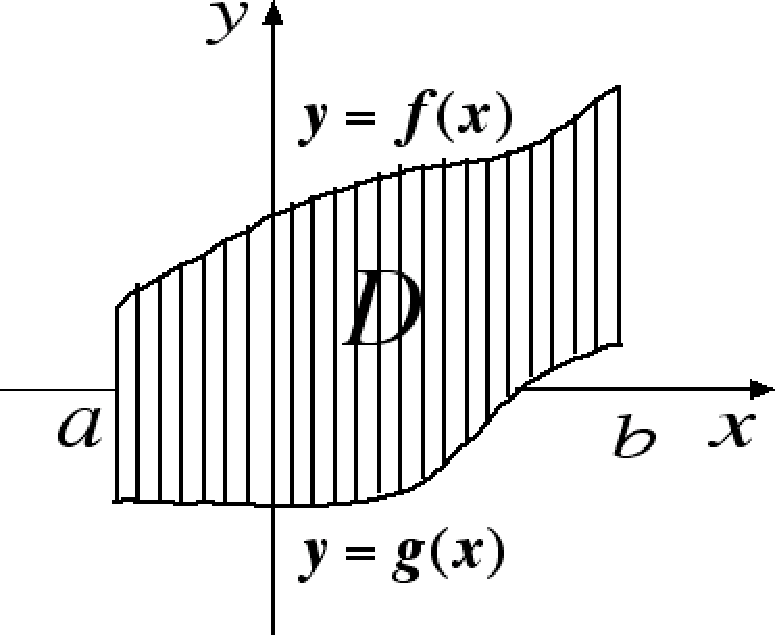
\includegraphics[width=6cm,height=4cm]{Figura1.pdf}
\caption{Aqui escrevemos a legenda desta figura.}
\label{fig:Figa}
\end{figure}
%%%%%

\newpage

\noindent
Tamb\'em podemos fazer doutra forma, por exemplo como na Figura \ref{fig:Figb}.
%%%%%
\begin{figure}[ht]\centering
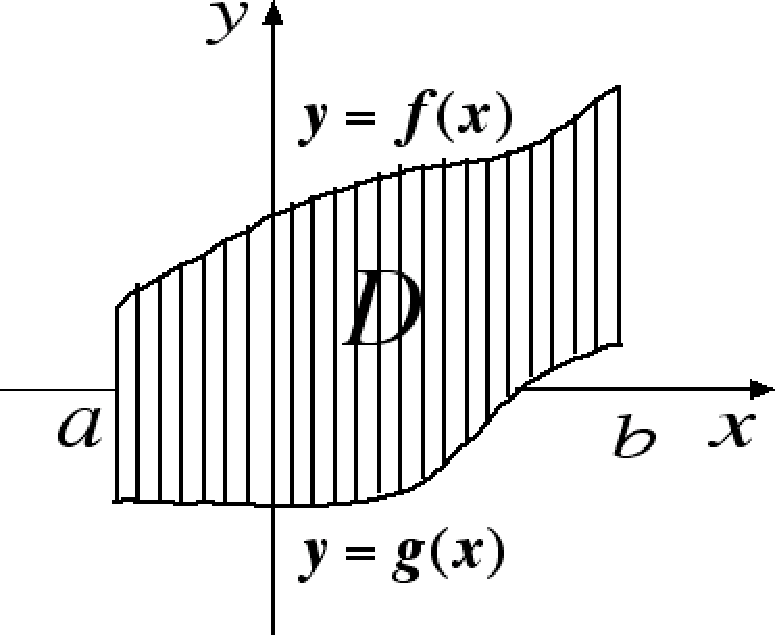
\includegraphics[height=3cm]{Figura1}   \hspace*{2cm}
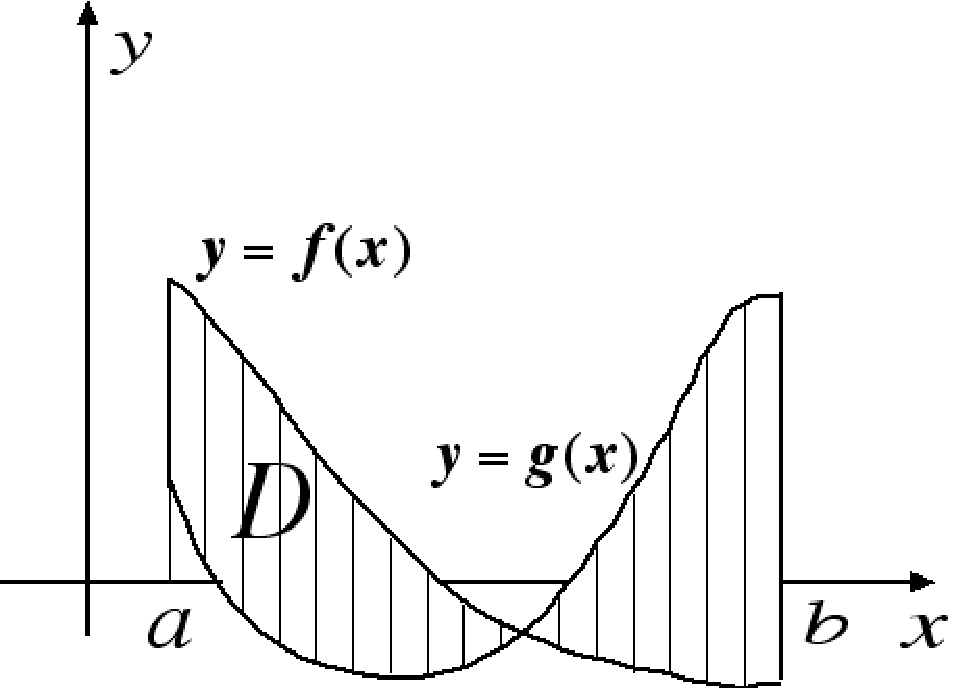
\includegraphics[height=5cm]{Figura2}
\caption{Aqui escrevemos a legenda desta figura.}
\label{fig:Figb}
\end{figure}
%%%%%

\noindent
Tamb\'em podemos fazer doutra forma, por exemplo como na Figura \ref{fig:Figc}.
%%%%%
\begin{figure}[ht]\centering
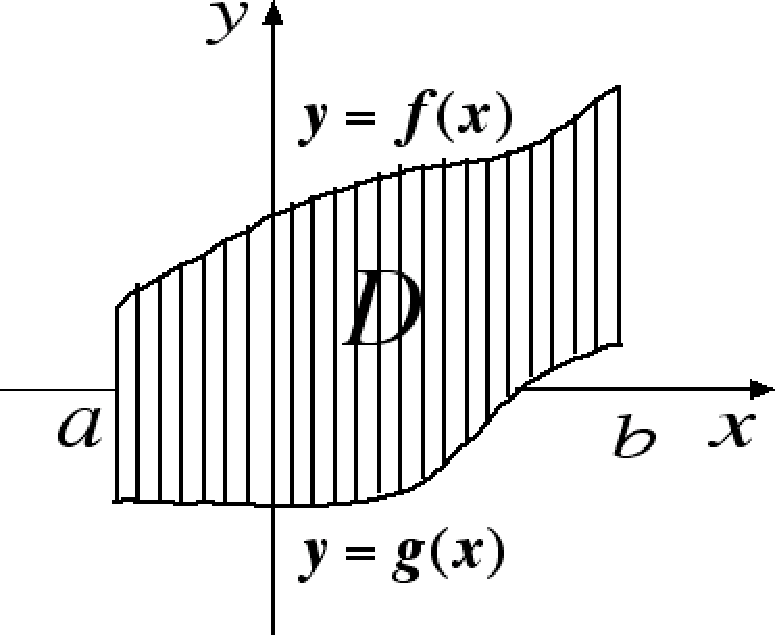
\includegraphics[height=3cm]{Figura1}   \hspace*{0.75cm}
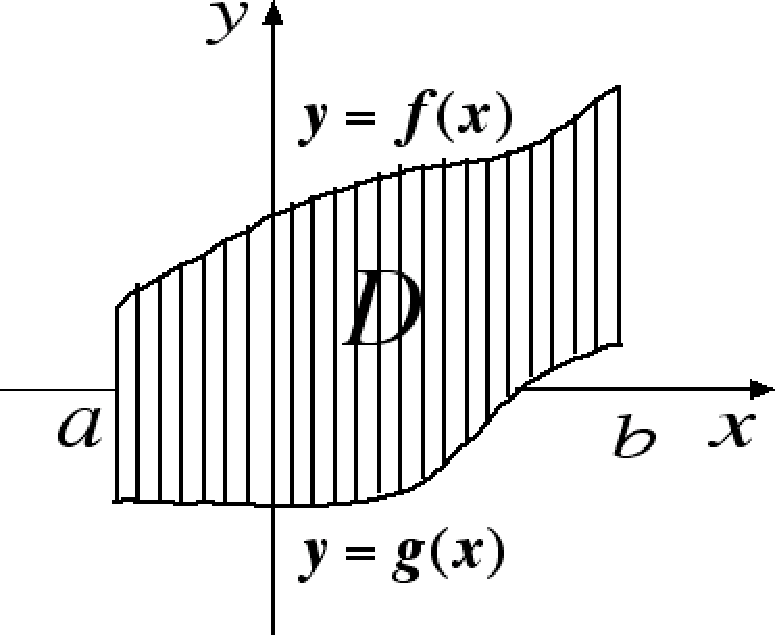
\includegraphics[height=4cm]{Figura1}   \hspace*{0.75cm}
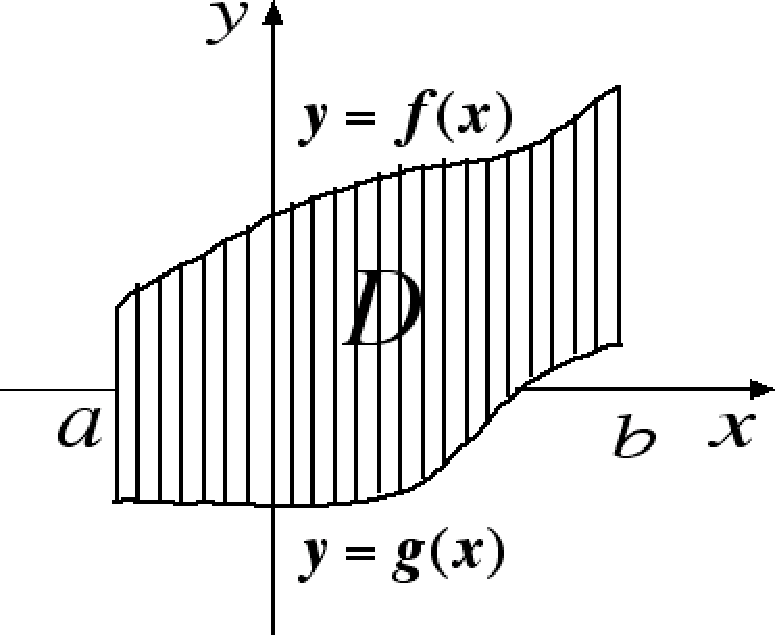
\includegraphics[height=2cm]{Figura1}
\caption{Aqui escrevemos a legenda desta figura.}
\label{fig:Figc}
\end{figure}
%%%%%

%%%%%%%%%%%%%%

\section{Conclus�o ou Coment\'arios finais}
\label{sec:Concl}


Registo de algum aspecto que n�o foi referido anteriormente e que possa ter interesse.
Por exemplo, uma breve refer�ncia a modelos relacionados com o modelo que se estudou.
Liga\c c\~oes entre os v\'arios modelos.
Estudos que foram realizados com aplica\c c\~ao do modelo ou de variantes do modelo.

\bigskip

\noindent
Para a Bibliografia, \'e conveniente usar automatismos, como se faz a seguir.

\noindent
Devo incluir Livros como em \cite{livro}, Artigos como em \cite{artigo}, Notas como em \cite{nota} \& Apontamentos.
Se tiver Teses, fa\c co como em \cite{tese} 
Outros textos de apoio.
Informa\c c\~ao dispon\'\i vel em {\it sites} de Internet, como em \cite{site}.
Etc.

\bigskip

\noindent
{\color{ggreen}Depois da Bibliografia, inclu\'\i \ f\'ormulas matem\'aticas e outras coisas \'uteis.}

%%%%%%%%%%%%%%

\begin{thebibliography}{99}

\bibitem{livro} 
A. Autor e B. Autor,
{\it T\'\i tulo do livro}, Wiley, New York, 2012.

\bibitem{artigo} 
A. Autor e B. Autor,
``T\'\i tulo do artigo na revista'', {\it Nome da Revista},  Vol.~000, No.~00 (2012), pp. 0000-0000.

\bibitem{nota} 
A. Autor, B. Autor e C. Autor,
``T\'\i tulo da Nota'', {\it T\'\i tulo da confer\^encia}, 
AMS Proceedings, Vol.~000, 2012, Eds. A.A.~Editor1, B.B.~Editor2, pp. 00-00.

\bibitem{tese} 
A. Autor,
``T\'\i tulo da tese'', Tese de Mestrado ou de Doutoramento, Universidade, Pa\'\i s, 2012.

\bibitem{site} 
Informa\c c\~ao que \`a data tal e tal estava dispon\'\i vel no seguinte site de categoria
\url{https://www.google.pt/}  

\end{thebibliography}


%%%%%%%%%%%%%%

\newpage

%%%%%%%%%%%%%%

\section{Tipos de letra e tamanhos diferentes}
\label{sec:varios}

{\sf Este \'e um tipo de letra.}

\medskip

\noindent
{\it E este \'e outro tipo de letra.}

\medskip

\noindent
{\bf E este \'e outro tipo de letra.}

\medskip

\noindent
$\cal A \ B \ C \ D \ E \ F \ G \ H \ I \ J \ K \ L \ M \ N \ O \ P \ Q \ R \ S \ T \ U \ V \ W \ X \ Y \ Z$

\medskip

\noindent
{\bf E este \'e outro tipo de letra.}

\medskip

\noindent
$\mathfrak{A}$ \ $\mathfrak{B}$ \ $\mathfrak{C}$ \ $\mathfrak{D}$ \ $\mathfrak{E}$ \ $\mathfrak{F}$

\medskip

\noindent
$\mathbb{A}$ \ $\mathbb{B}$ \ $\mathbb{C}$ \ $\mathbb{D}$ \ $\mathbb{E}$ \ $\mathbb{F}$

\bigskip \bigskip

\noindent
{\large\bf Diferentes tamanhos}

\medskip

\noindent
{\tiny Muito pequeno} \qquad
{\scriptsize N\~ao t\~ao pequeno}\qquad
{\footnotesize Ainda \' e pequeno}\qquad
{\normalsize Tamano normal}\qquad

\medskip

\noindent
{\large Agora vai aumentando}\qquad
{\Large E fica maior}\qquad
{\LARGE E maior ainda}

\medskip

\noindent
{\huge E muito maior}\qquad
{\Huge Imenso imenso}


%%%%%%%%%%%%%%

\newpage

%%%%%%%%%%%%%%

\section{Coisas variadas de texto matem\'atico}
\label{sec:mat}

Algumas instru\c c\~oes \'uteis s�o apresentadas de seguida.

\

%%%%%%

\noindent
{\bf Equa\c c\~ao sem n\'umero}

$$
\frac{1}{3x} = \sqrt{57} + \cos 2\theta \int_{-3}^{+\infty} x^3 \sen 2x \, dx
$$

%%%%%%

\noindent
{\bf Equa\c c\~ao com n\'umero}

\begin{equation}
\frac{1}{3x} = \sqrt{57} + \cos 2\theta \int_{-3}^{+\infty} x^3 \sen 2x \, dx
\label{eq:peixe}
\end{equation}
e depois, se eu  quiser chamar a equa\c c\~ao, escrevo, por exemplo,
que a partir da Eq. (\ref{eq:peixe})
se pode deduzir o resultado esperado.

\medskip

%%%%%%

\noindent
{\bf Sistema de equa\c c\~oes sem n\'umero}

$$
\left\{
\begin{array}{l}
x u_x - y u_y = x^2 + y^2 ,   \quad (x,y) \in \RR^2  \medskip  \\
u(s^3,s^5) = s^2 + 1 , \quad s \in \RR
\end{array}
\right.
$$

\medskip

%%%%%%

\noindent
{\bf Sistema de equa\c c\~oes com n\'umero}

\begin{equation}
\left\{
\begin{array}{l}
x u_x - y u_y = x^2 + y^2 ,   \quad (x,y) \in \RR^2  \medskip  \\
u(s^3,s^5) = s^2 + 1 , \quad s \in \RR
\end{array}
\right.
\end{equation}

\bigskip

%%%%%%

\noindent
{\bf Tabela}

\begin{table}[h!]

\vspace*{0.25cm}

\begin{center}
\begin{tabular}{| c | c | c | c |}
\hline \hline
  &  {\small Estado $S$}   &   {\small Estado $N$}   &  {\small Estado $I$} 
\\ \hline \hline
$n_1$  &  $0.30112$ & $0.10590$  & $0.03000$ 
\\ \hline
$n_2$  &  $0.27563$ & $0.07060$  & $0.02000$ 
\\ \hline
$n_3$  &  $0.03014$ & $0.35300$  & $0.10000$ 
\\ \hline
$n_4$  &  $0.28496$ & $0.70601$  & $0.20000$ 
\\ \hline\hline
$n $  &  $0.89185$ & $1.23551$  & $0.35000$ 
\\ \hline
$T $  &  $2363.16$ & $2357.89$  & $298.15$
\\ \hline
$v $  &  $2126.46$ & $2508.51$  & $0$
\\ \hline \hline 
%%%%%
\end{tabular}
\end{center}
\label{tab1}
\caption{Aqui escrevo a legenda desta tabela.}
\end{table}

\bigskip

%%%%%%

\noindent
{\bf Bloco de equa\c c\~oes}
\begin{eqnarray}
& & \hspace*{-1cm}
        \frac{\partial n_\alpha}{\partial t}  \!+\!
        \nabla \! \cdot \! {\left(n_\alpha \u_\alpha \right)} =  \tau_\alpha ,
        \; \alpha=1,\ldots,4 
        \label{roi}
        \\  \nonumber  \\
& & \hspace*{-1cm}
        \frac{\partial}{\partial t} (\varrho\v) \!+\! \nabla  \! \cdot \!
        {\left(\varrho\v\otimes\v+\PP\right)} = 0 
        \label{mom}
        \\  \nonumber  \\
& &  \hspace*{-1cm}
        \frac{\partial}{\partial t}
        \Big( \frac32nk_BT  \!+\!  \sum_{\alpha =1}^4n_ \alpha \varepsilon_\alpha  \!+\!  \frac12\varrho\v^2\Big)
         \!+\!   \nabla  \! \cdot \! \Big[ \q  \!+\!  \PP \v \quad
         \nonumber  \\
& &   \hspace*{1cm}+
         \Big( {3\over 2}nk_BT \!+\! \sum_{\alpha =1}^4n_ \alpha \varepsilon_\alpha \!+\! \frac12\varrho\v^2\Big)\v\Big] \!=\! 0 
         \label{en}
\end{eqnarray}


\bigskip \bigskip \bigskip


\noindent
Na Internet h\'a muitos manuais de \LaTeX,
por exemplo

\bigskip \bigskip

\noindent
\url{http://zelmanov.ptep-online.com/ctan/lshort_port.pdf}

\end{document}








